\documentclass[12pt]{article}
\usepackage{amsmath}
\usepackage{graphicx}
\usepackage{hyperref}
\usepackage[latin1]{inputenc}
\usepackage{float}
\usepackage[a4paper, portrait, margin=0.5in]{geometry}

\graphicspath{ {../} }

\title{CS547 Assignment 2\\Project Cost Estimation}
\author{Wojciech Cichoradzki\\201506554}
\date{01/12/2019}

\begin{document}
\maketitle

\section{Abstract}
A Python 3 script was implemented which goal is to find appropriate function that takes a set to inputs and returns predicted development cost of the project (effort) using genetic programming approach. Three different datasets were evaluated and compared against non-genetic programming approach that used linear regression. This reports consists of the analysis of the solutions of three datasets:
\begin{enumerate}
  \item Albrecht dataset consisting of 7 inputs and 24 records
  \item Kemerer dataset consistsing of 6 inputs and 16 records
  \item China dataset consisting of 16 inputs and 499 records
\end{enumerate}
The results show better performance of genetic programming approach compared to linear regression for given dataset.

\section{Methodology}

\subsection{Genetic Programming configuration}
Each dataset was evaluated using similar configuration of the script. Configurations for each datasets are stored inside the \texttt{configs} directory. The shared configuration for all genetic programming tests included:
\begin{itemize}
  \item Mating chance - 50\%
  \item Mutation chance - 20\%
  \item Number of generations - 1000
  \item Population size - 200
  \item Depth limit of the syntax tree - 20
\end{itemize}
Moreover each dataset was split so part of the dataset was used to train the model while the rest was used for validation testing. The train/test split for each dataset was as follows:
\begin{enumerate}
  \item Albrecht: 70/30 \%
  \item Kemerer 66/34 \%
  \item China 66/34 \%
\end{enumerate}
Test data was processed to include only meaningful inputs (e.g. exluding ID numbers).
When it comes to function syntax generation the following primitives and constants were allowed to be generated:
\begin{enumerate}
  \item Addition of 2 elements
  \item Subtraction of 2 elements
  \item Multiplication of 2 elements
  \item Negation of 1 element
  \item Random ephemeral integer constant from the set of $\{-1, 0, 1\}$
  \item Random ephemeral float constant between -1 and 1 rounded to 3 decimal points.
\end{enumerate}
\subsubsection{Prediction metric}
To evaluate validity of the candidate solution the Mean Magnitude of Relative Error (MMRE) metric was used calculated as follows:
\begin{equation}
  MMRE=\frac{\sum\limits_{i=1}^N \frac{|f_a(i) - f_p(i)|}{f_a(i)}}{N}
\end{equation}
where $N$ is the size of test data, $i$ is test number, $f_a(i)$ is the actual result for $i^{th}$ test, $f_p(i)$ is the predicted results for the $i^{th}$ test. This value was then fed as the fitness function result to the genetic programming solver as a minimizer function.

\subsection{Linear regression comparison metric}
Linear regression comparison was evaluated using weka software using same test/train split setting as for respectful tests performed in the genetic programming part. The predicted values for test data were then evaluated later in MS Excel to calculate the $MMRE$ since weka is not providing this metric out of the box. All the weka-related results are stored in the \texttt{/results/<test-name>/weka} directories.

\section{Evaluation of results}

\subsection{Albrecht dataset}

\begin{figure}[H]
  \centering
  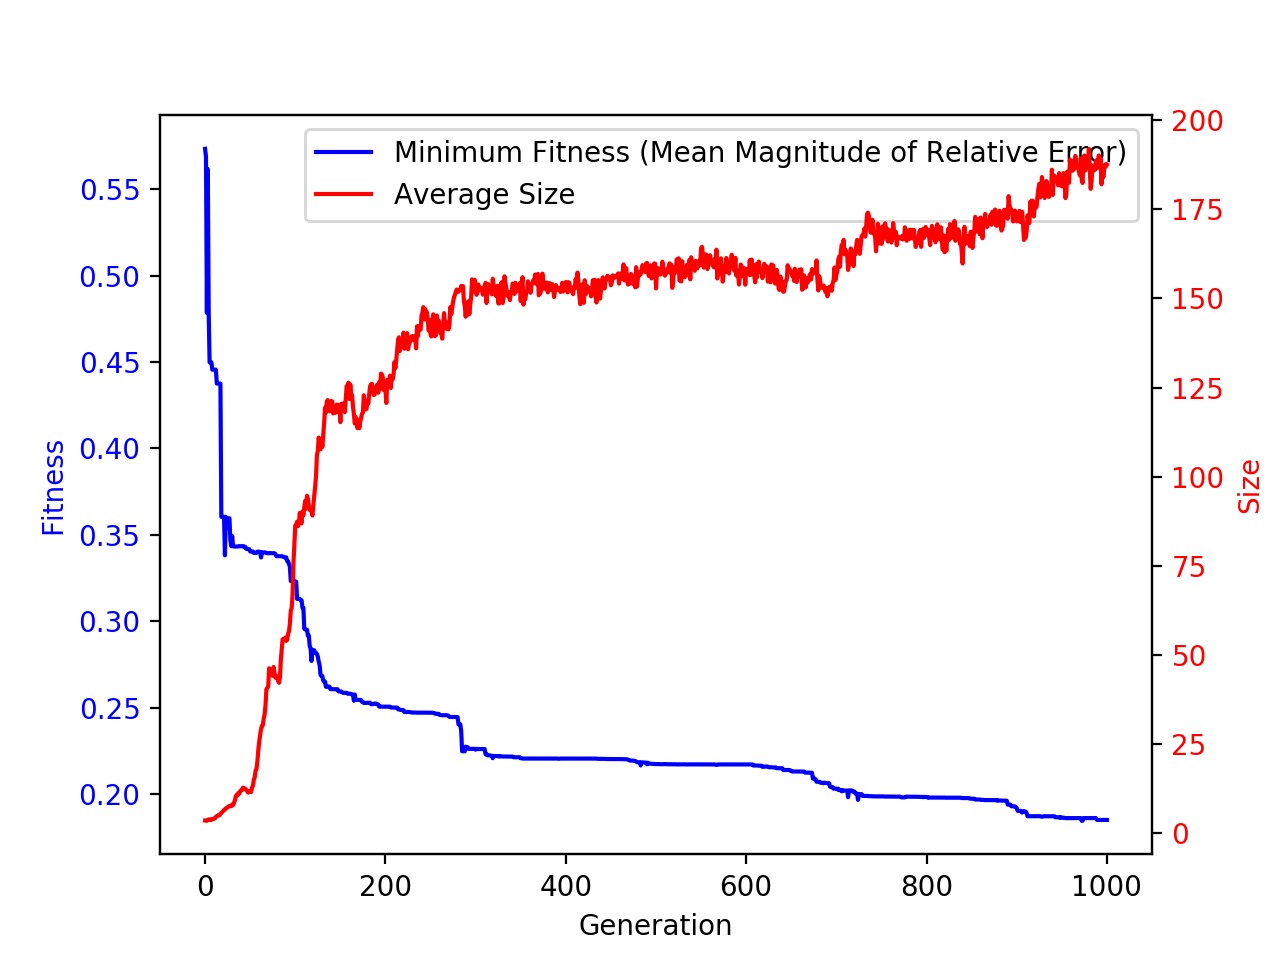
\includegraphics[width=0.8\textwidth]{results/albrecht/mmre_vs_size}
  \caption{Fitness vs syntax tree size over generations in genetic programming approach}
  \label{fit_vs_syn_albrecht}
\end{figure}
As seen in fig. \ref{fit_vs_syn_albrecht}, genetic programming approach on the train data achieved quick decrease in the $MMRE$ value over first 100 generations alongside rapid growth of the syntax tree size to over 100 nodes. Over the next generations, until the ending point, it reached the minimum of under 20\% mean magnitude of relative error and around 185 nodes in the return function.

\begin{figure}[H]
  \centering
  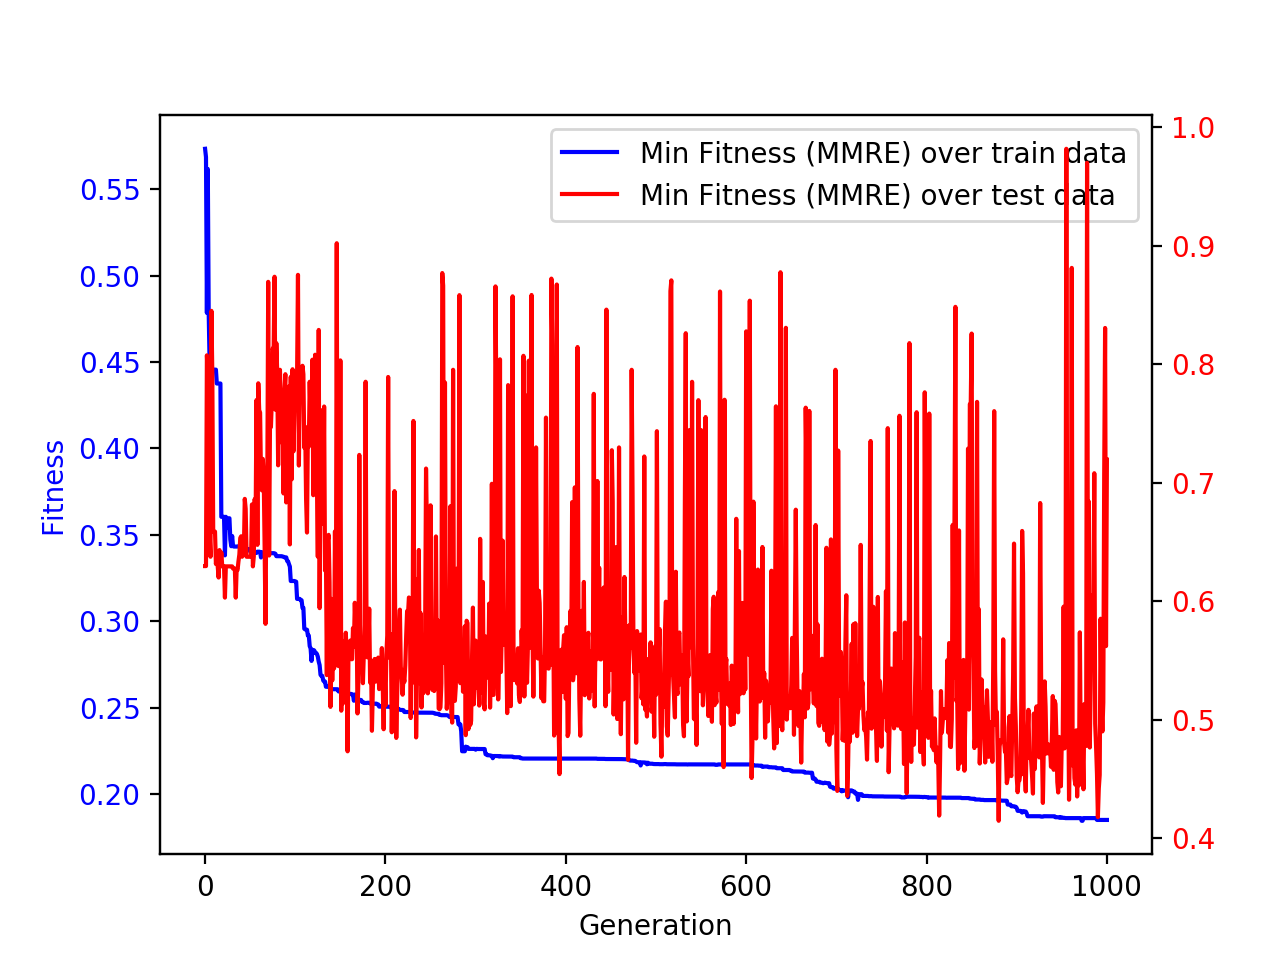
\includegraphics[width=0.8\textwidth]{results/albrecht/mmre_train_vs_test}
  \caption{Comparison of MMRE on test and train data over generations}
  \label{train_test_albrecht}
\end{figure}
Next, the result function was compared against train and test data in fig.\ref{train_test_albrecht}. MMRE over test data was varying greatly as the model was trained hence generating a lot of noise on the graph. Nevertheless, it can be noticed that the average curve over test data was also decreasing over generations as the model was trained resulting at best around 40\% - 50\% MMRE. The spike at the end of the graph at roughly $950^{th}$ generation may be a result of overfitting the function on train data.

\begin{figure}[H]
  \centering
  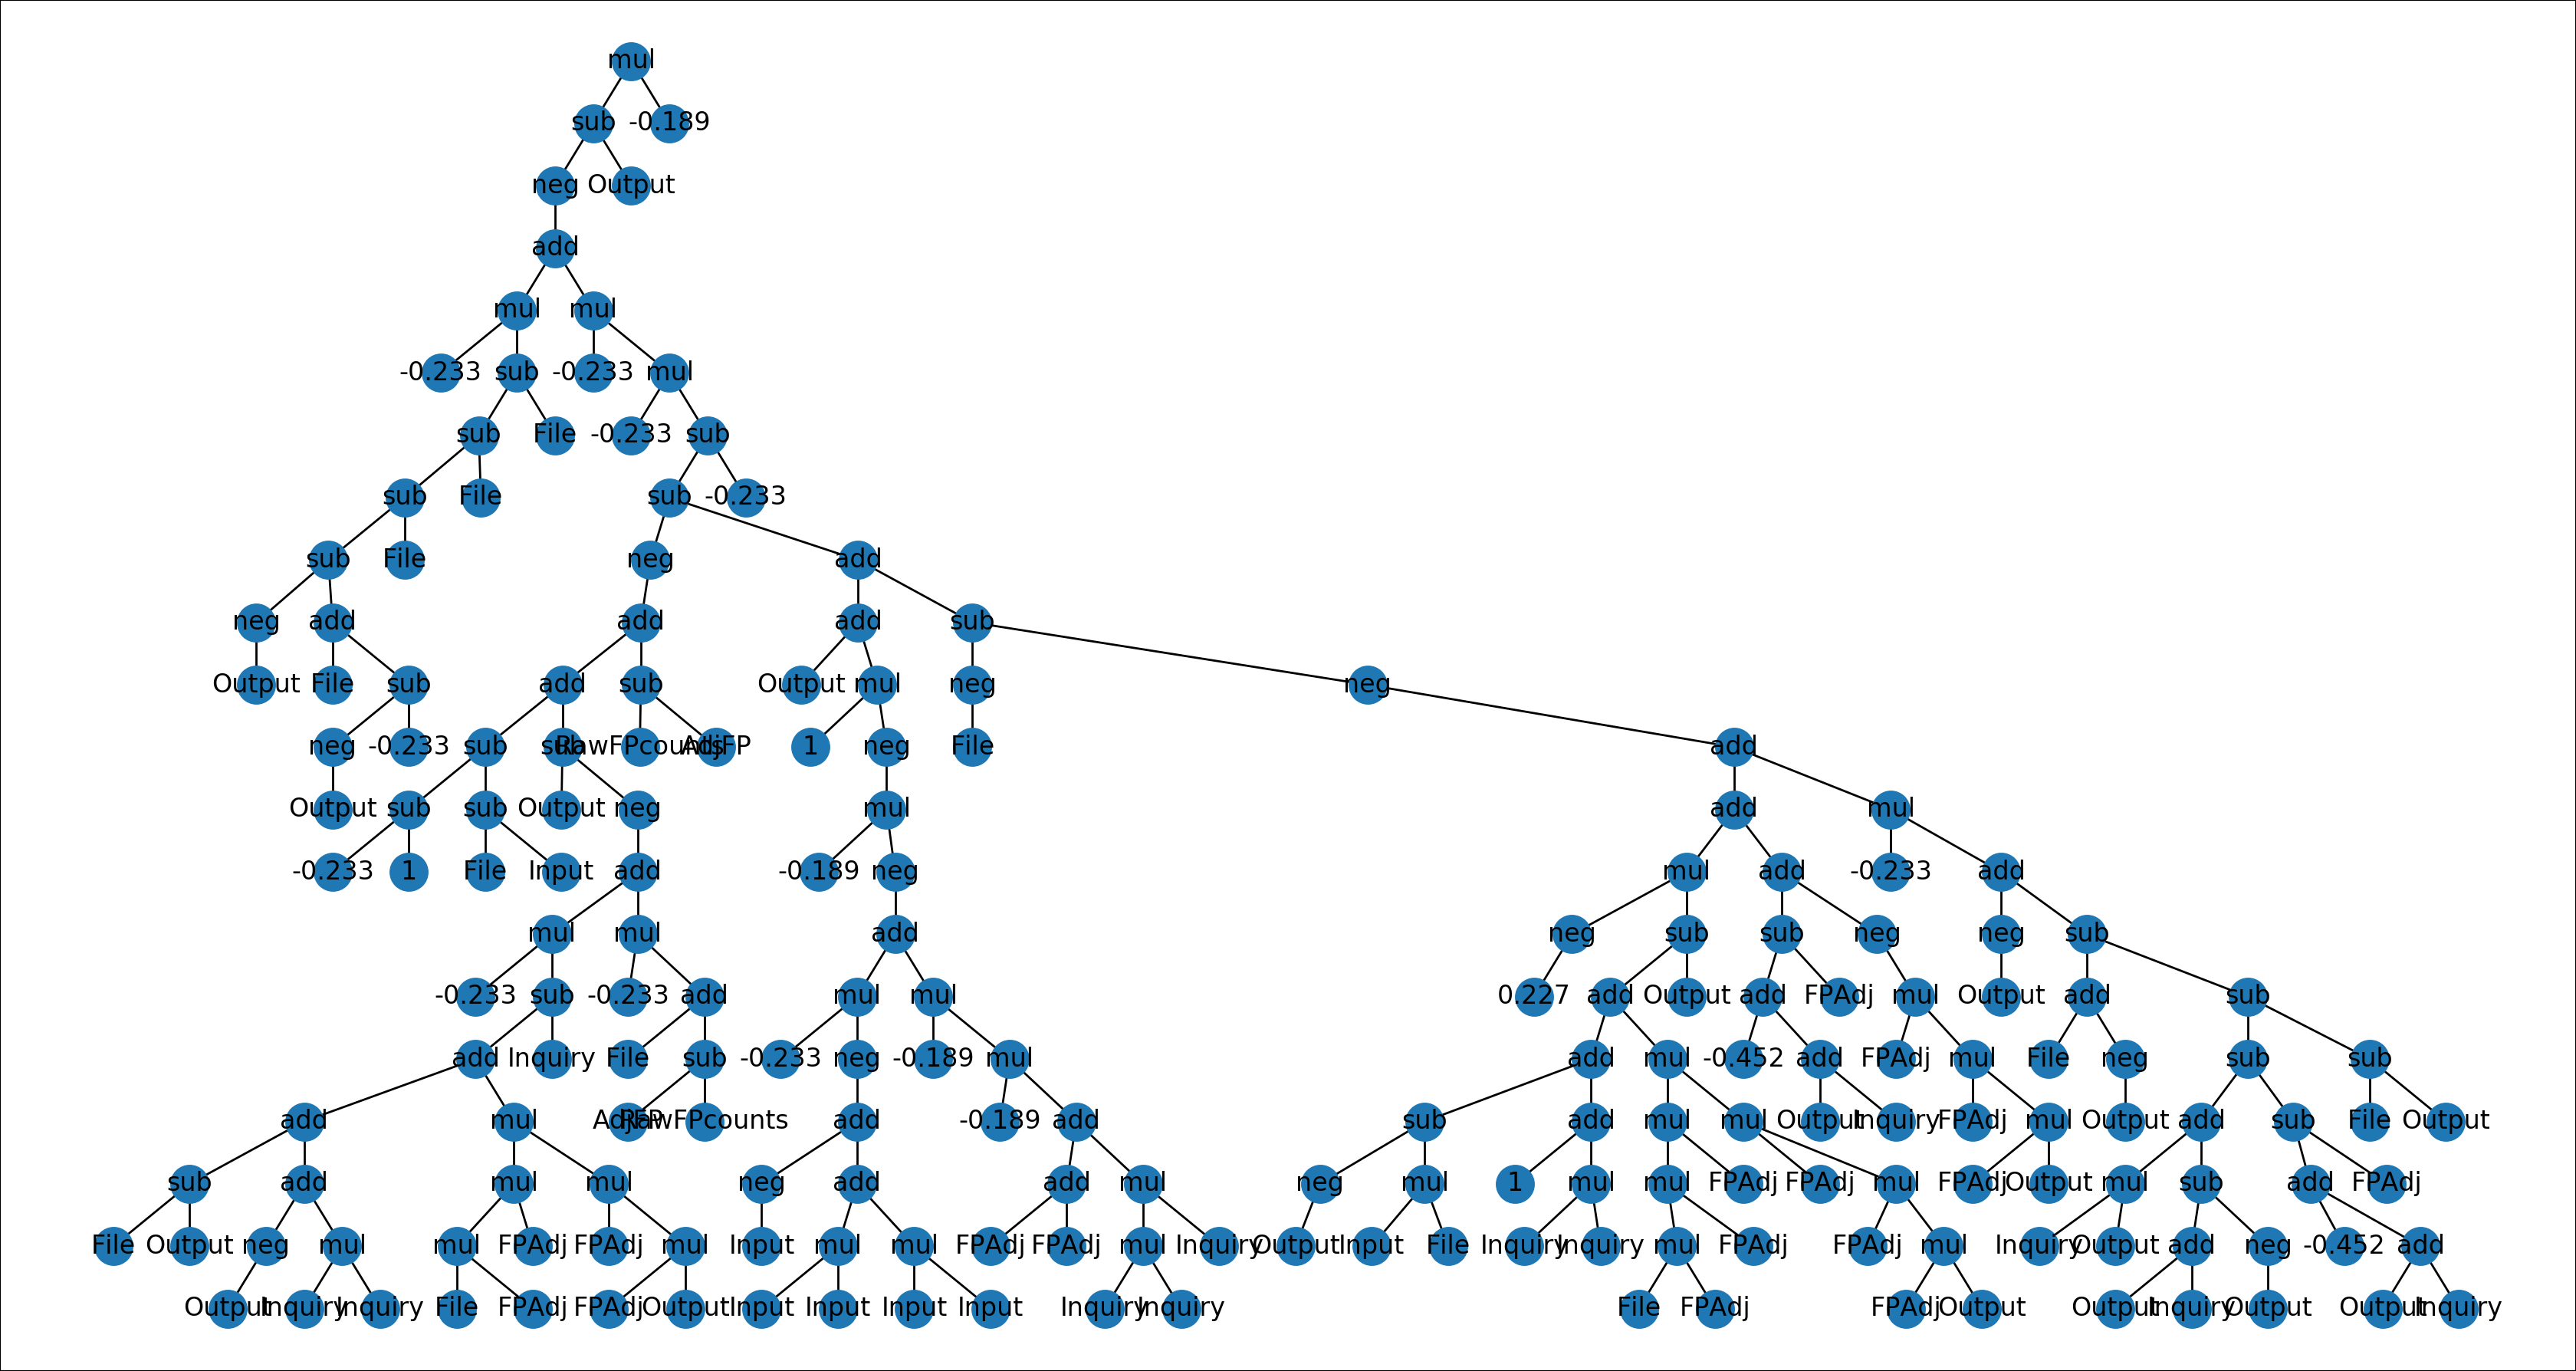
\includegraphics[width=0.8\textwidth]{results/albrecht/test_function}
  \caption{Syntax tree graph of the best resulting function for the albrecht dataset}
  \label{function_albrecht}
\end{figure}

Nevertheless, the albrecht dataset was too small to find the well-performing approximation model, the best function that the genetic programming solver came up with can be seen above in fig. \ref{function_albrecht}. It consists of over 150 nodes and reached the limit of 20 levels depth. Due to this limit, it could be a blocking factor fo the function to evolve further and yield better results.

Lastly, the results from running weka linear's regression classifier yielded much simpler function:
\begin{equation}
  Effort = 0.405  * Output -2.2232
\end{equation}
The resulting MMRE over test data of the linear regression solution equaled to 49.78\% which is within the upper limit of the best performing genetic programming solutions.

As a result, both genetic programming and linear regression classified provided somewhat comparable solutions with the mean magnitude of relative error at around 50\%. This magnitude of error is very large and as such is not suitable for any further practical usage for project cost estimation. Genetic programming solutions were slightly outperforming linear regression ones, however it took them significantly more time.
In order to improve the results with the genetic algorithm, one could try expanding the limit of 20 depth, as my machine was performing very slowly when this limit was incrased. With even larger search space, and ideally larger train dataset, genetic programming might have outperfomed linear regression classifier.

\subsection{Kemerer dataset}

\begin{figure}[H]
  \centering
  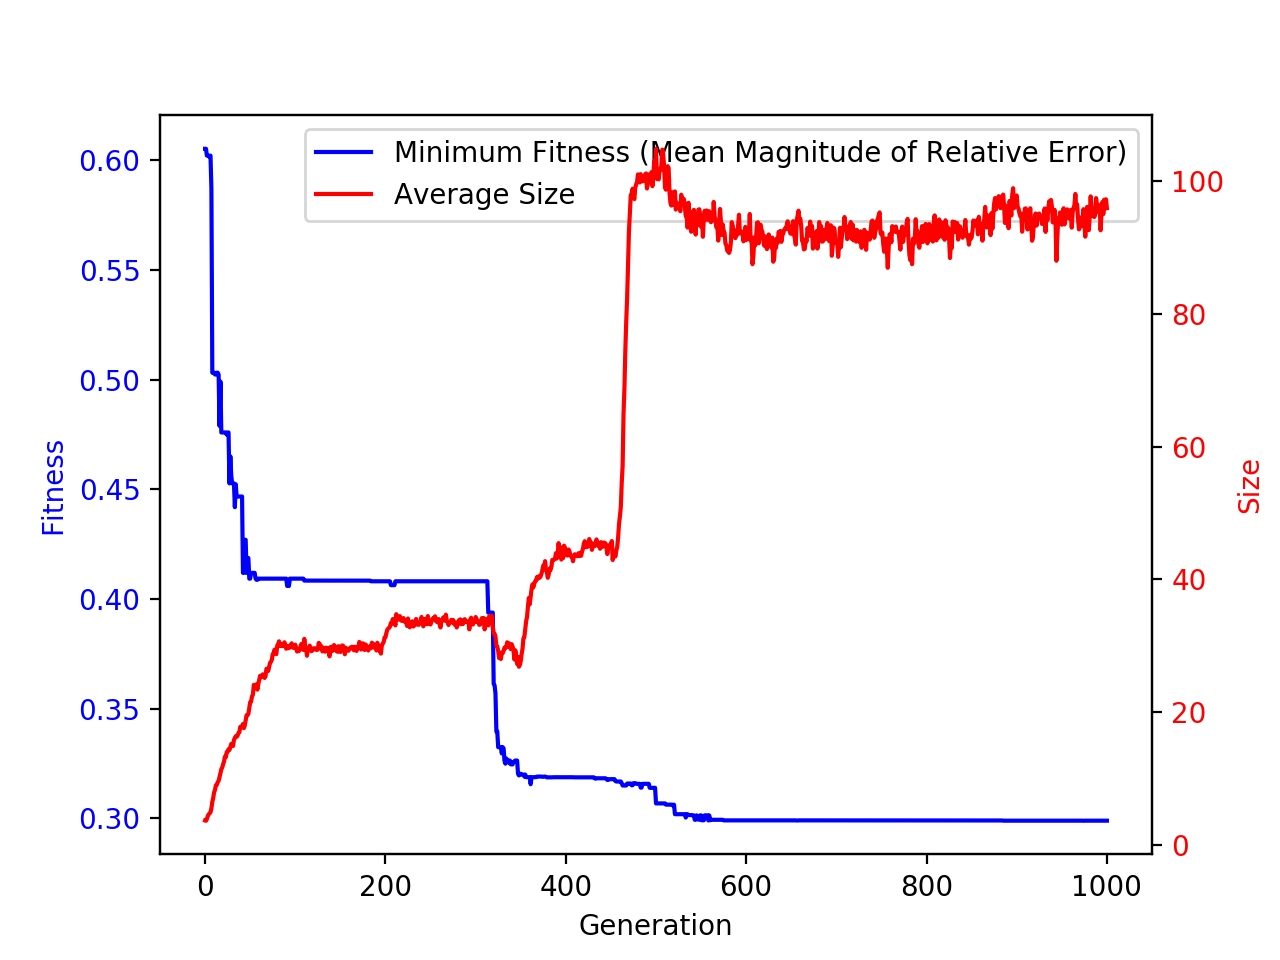
\includegraphics[width=0.8\textwidth]{results/kemerer/mmre_vs_size}
  \caption{Fitness vs syntax tree size over generations in genetic programming approach}
  \label{fit_vs_syn_kemerer}
\end{figure}
As seen in fig. \ref{fit_vs_syn_kemerer}, genetic programming approach on the kemerer train data again achieved quick decrease in the $MMRE$ value over first 50 generations, then it stagnated for about 200 generation only to jump with a decrease by about 0.1 MMRE before generation 400. After generation 600, it maintained same fitness value until the end of experiment, resulting in the final minimum mean magnitude of relative error metric at around 30\% on train data and the size of the syntax tree of roughly 100 nodes.

\begin{figure}[H]
  \centering
  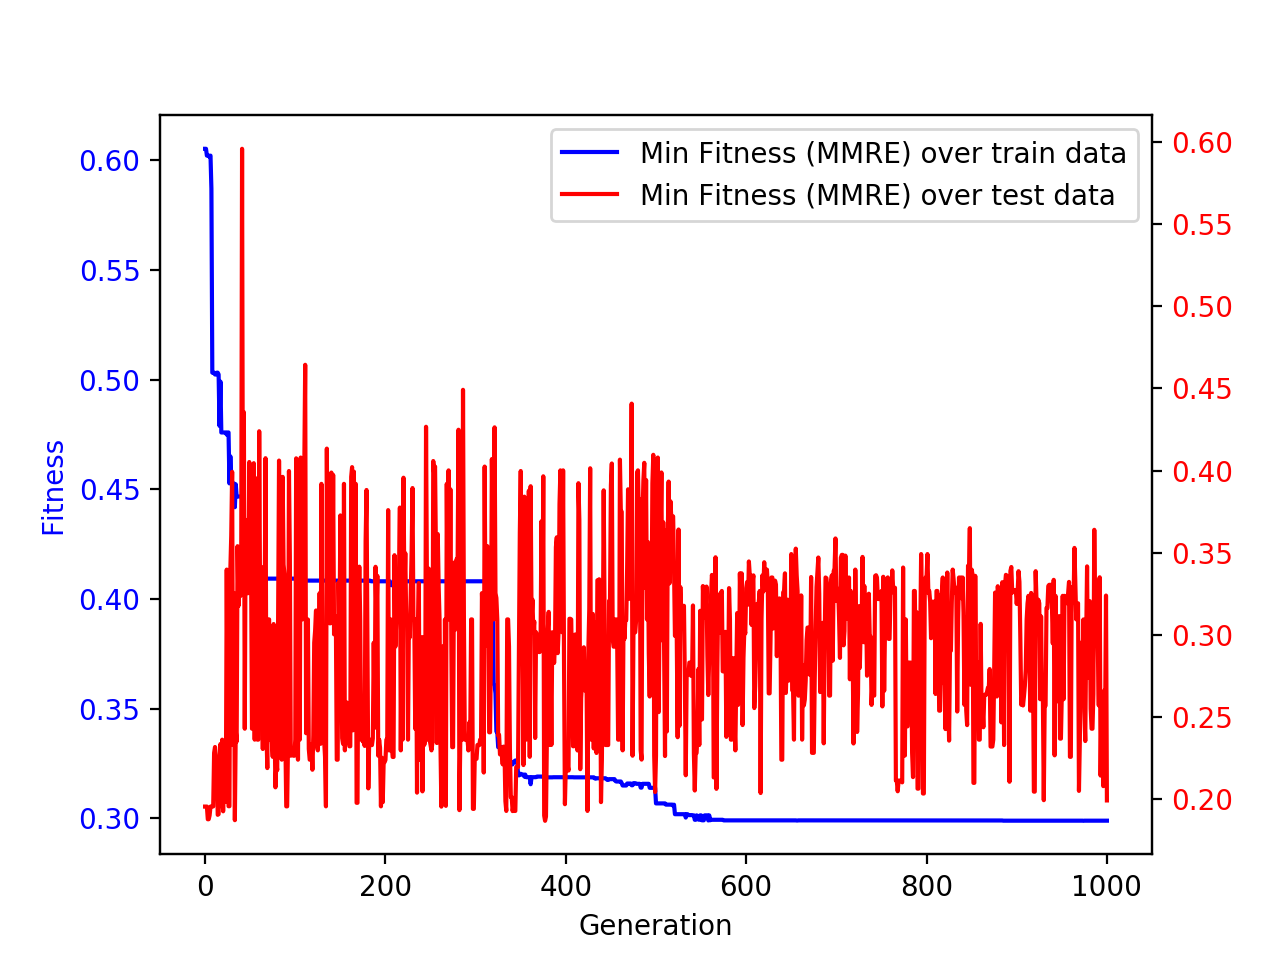
\includegraphics[width=0.8\textwidth]{results/kemerer/mmre_train_vs_test}
  \caption{Comparison of MMRE on test and train data over generations}
  \label{train_test_kemerer}
\end{figure}
As seen in fig. \ref{train_test_kemerer} MMRE over test data was varying between 40-20\% until the stagnation after 600 generations when it reached the range between 35-20\%.

\begin{figure}[H]
  \centering
  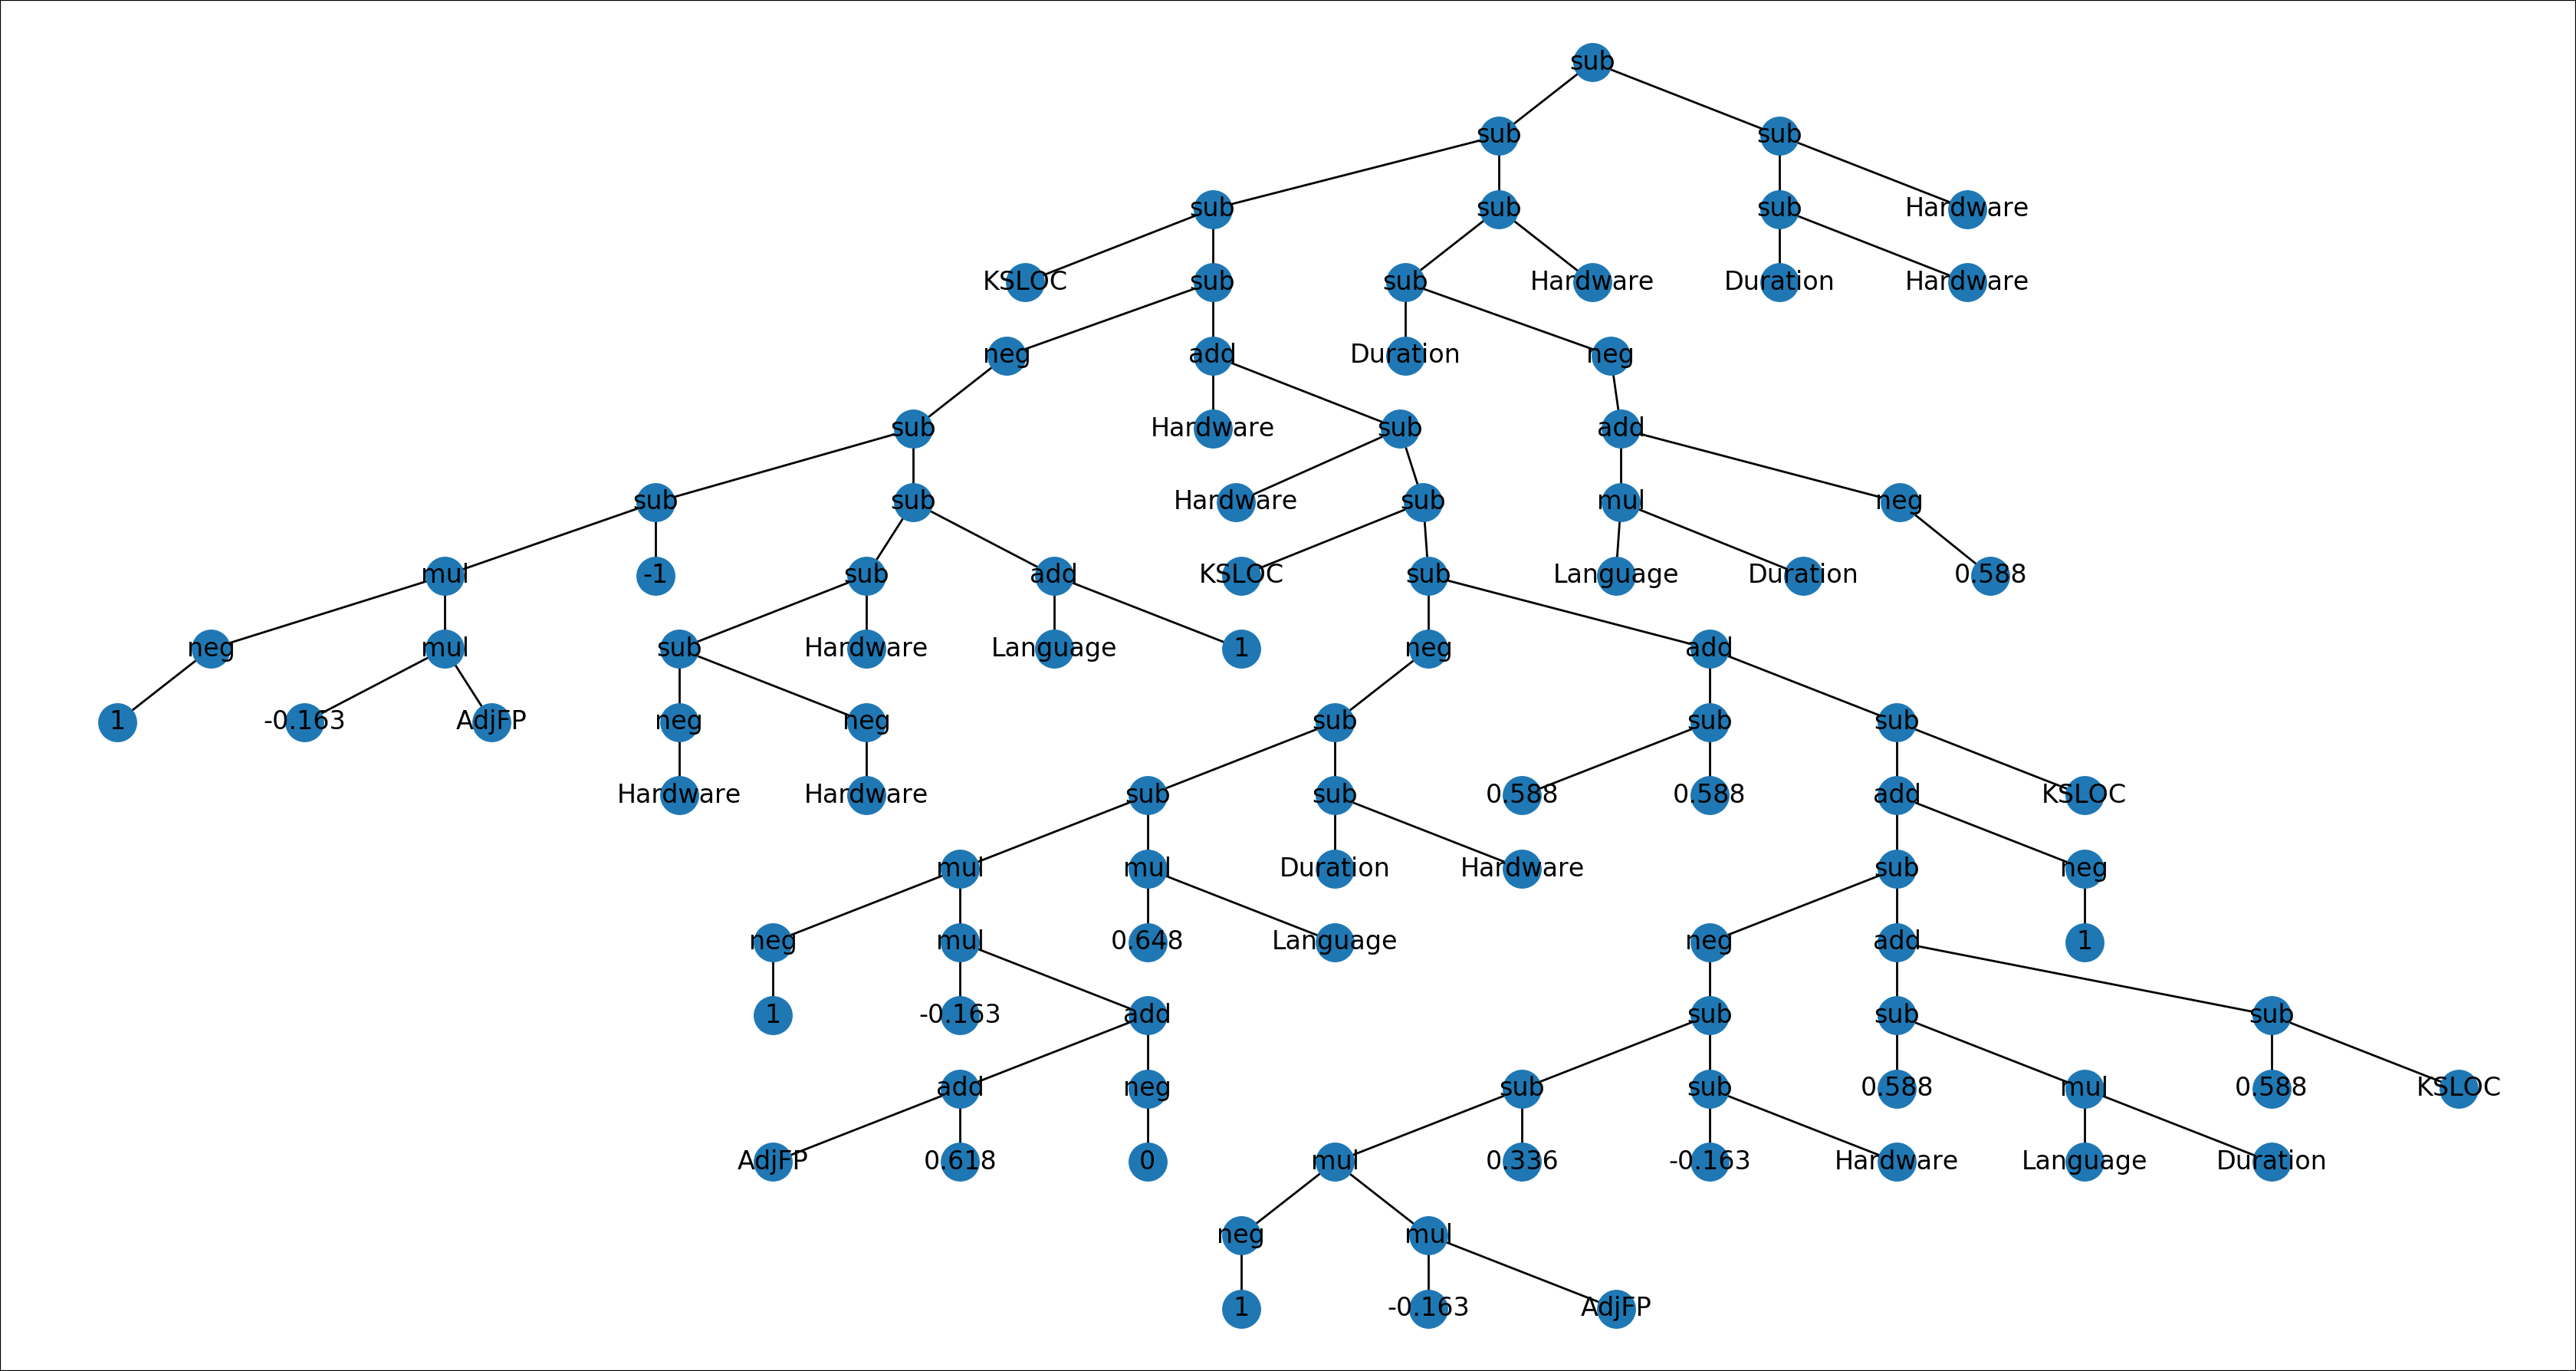
\includegraphics[width=0.8\textwidth]{results/kemerer/test_function}
  \caption{Syntax tree graph of the best resulting function for the kemerer dataset}
  \label{function_kemerer}
\end{figure}

The generated effort function is much cleaner compared to albrecht dataset result, while still being much more complex comparing against the generated by weka's linear's regression function:
\begin{equation}
  Effort = 80.9791 * Hardware + 0.4557 * AdjFP -445.5517
\end{equation}
In this case, the resulting MMRE of the linear regression solution equaled to the whopping 111.83\% which is 4 to 6 times larger value than the genetic programming solution.

As a result, it the case of kemerer dataset, genetic programming yielded a much more optimal solution than the weka's linear regression classifier. It could be due to the larger search space and the non-polynomial result of the optimal effort function.

\subsection{China dataset}

\begin{figure}[H]
  \centering
  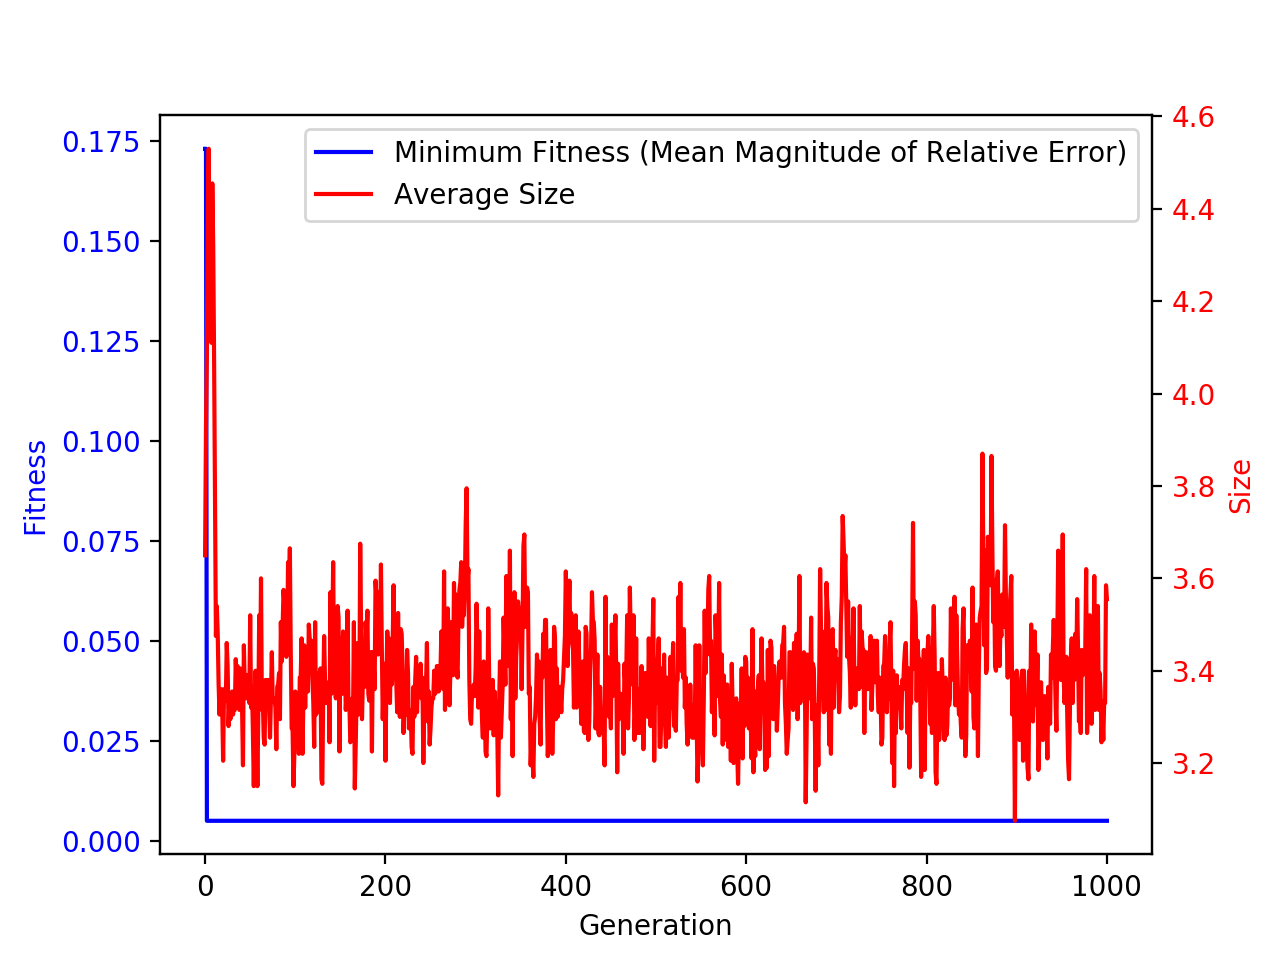
\includegraphics[width=0.8\textwidth]{results/china/mmre_vs_size}
  \caption{Fitness vs syntax tree size over generations in genetic programming approach}
  \label{fit_vs_syn_china}
\end{figure}
As seen in fig. \ref{fit_vs_syn_china}, a very interesting situation occured when running genetic programming solver against the china dataset. In the second generation, the almost-error-prone solution was found that resulted in the MMRE of just over 0.5\% and the size of just 3 nodes!. Over the next 998 generations, the program could not come up with anything better.

\begin{figure}[H]
  \centering
  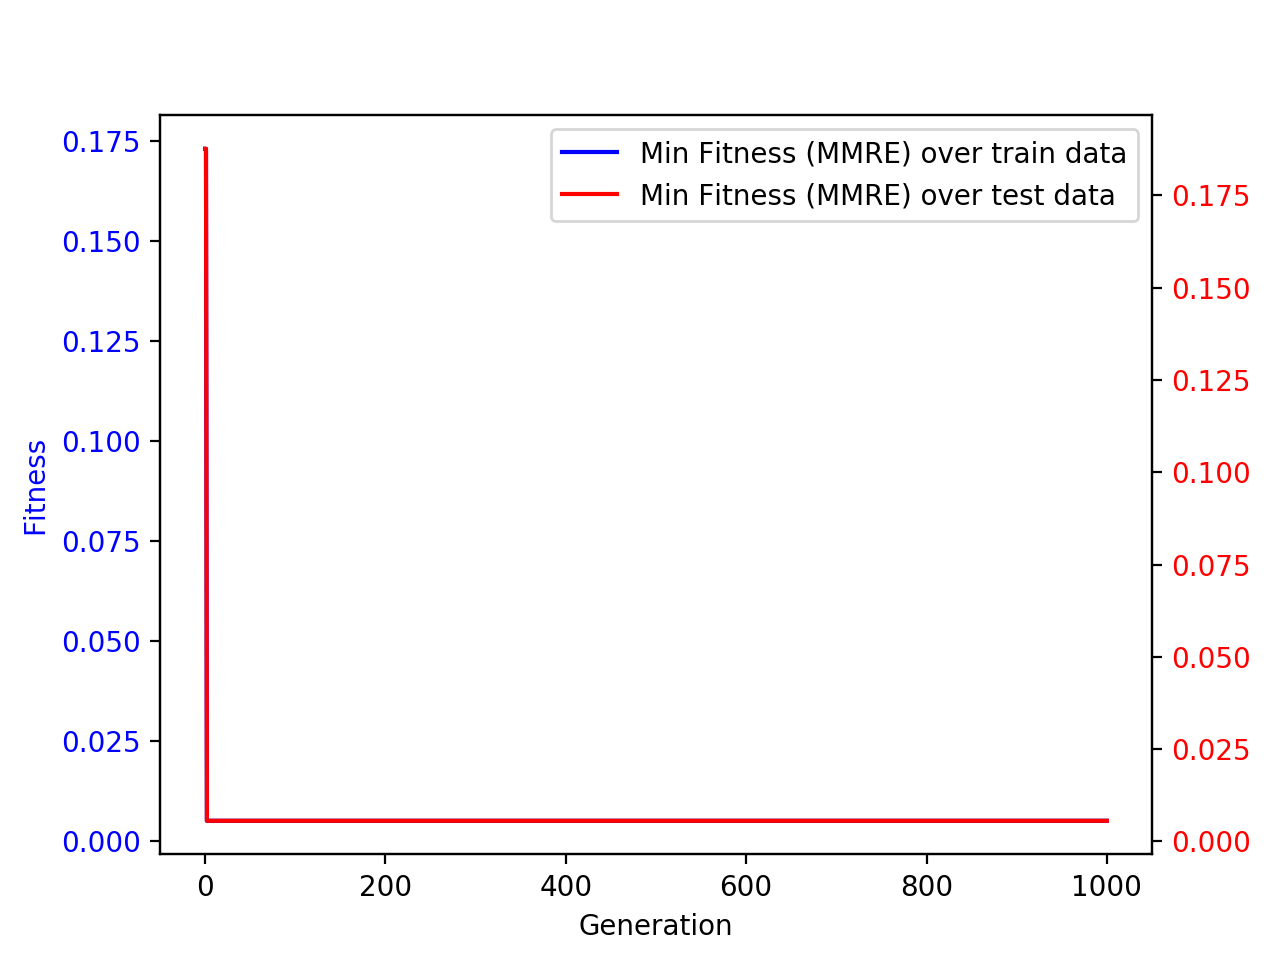
\includegraphics[width=0.8\textwidth]{results/china/mmre_train_vs_test}
  \caption{Comparison of MMRE on test and train data over generations}
  \label{train_test_china}
\end{figure}
Even more interestingly, the resulting function yielded identical result against test data. That means that the function is in clear correlation to the effort result.

\begin{figure}[H]
  \centering
  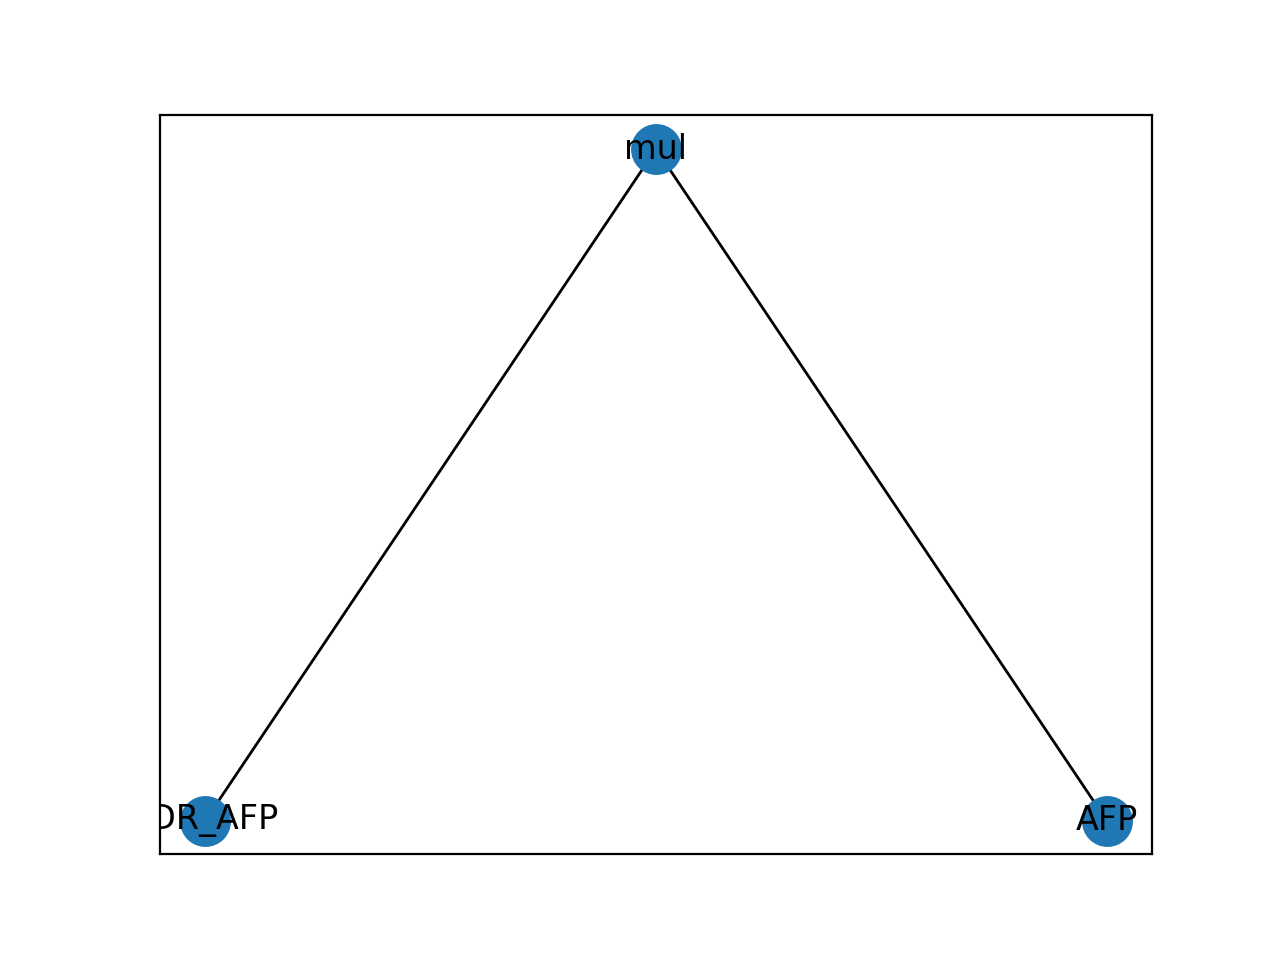
\includegraphics[width=0.8\textwidth]{results/china/test_function}
  \caption{Syntax tree graph of the best resulting function for the china dataset}
  \label{function_china}
\end{figure}

As seen in fig. \ref{function_china}, the effort function is simply two (out of 16 in total) inputs multipled together.
The function that weka classifier came up with is much more complex:
\begin{equation}
  \begin{array}{l}
    Effort = \\
    -0.0027 * Input + \\
     0.022  * Enquiry + \\
    -0.013  * File + \\
     0.0191 * Interface + \\
     0.0059 * Added + \\
     0.5822 * PDR\_AFP + \\
    -0.2798 * PDR\_UFP + \\
    -0.2209 * NPDR\_AFP + \\
     1.1732 * Resource + \\
     3.9372
  \end{array}

\end{equation}
In this case, the resulting MMRE of the linear regression solution equaled to 64.38\% which is vastly larger than <1\% from the genetic programming solution.

As a result, it the case of the china dataset, genetic programming created an almost-optimal solution very quickly. However, it has to be noted that there is a possibility than the effort in the china dataset could be actually a result of the \texttt{DR\_AFP * AFP} and the relative error comes from the floating-point arithmetic error. If that's the case, these two inputs should have been excluded from the search.

\end{document}
